% ============================================================
%  Grover's Quantum Search Algorithm — Detailed Lecture Notes
% ============================================================
\documentclass[12pt,a4paper]{article}

%% ── Core packages ───────────────────────────────────────────
\usepackage[margin=2.5cm]{geometry}
\usepackage{amsmath,amssymb,amsthm}
\usepackage{mathtools}
\usepackage{braket}          % Dirac: \ket{}, \bra{}, \Braket{}
\usepackage{xcolor}
\usepackage{tikz}
\usetikzlibrary{arrows.meta,shapes.geometric,positioning,
                decorations.pathreplacing,calc,angles,quotes,
                patterns,backgrounds}
\usepackage{pgfplots}
\pgfplotsset{compat=1.18}
\usepackage{tcolorbox}
\tcbuselibrary{theorems,skins,breakable}
\usepackage{booktabs}
\usepackage{array}
\usepackage{enumitem}
\usepackage{float}
\usepackage{caption}
\usepackage{subcaption}
\usepackage{cancel}
\usepackage{mdframed}
\usepackage{fancyhdr}
\usepackage{titlesec}
\usepackage{hyperref}
\hypersetup{colorlinks=true,linkcolor=qblue,urlcolor=qblue}

%% ── Colours ─────────────────────────────────────────────────
\definecolor{qblue}{RGB}{20,90,170}
\definecolor{qred}{RGB}{190,30,30}
\definecolor{qgreen}{RGB}{10,130,50}
\definecolor{qpurple}{RGB}{110,20,150}
\definecolor{qorange}{RGB}{205,95,0}
\definecolor{lightblue}{RGB}{218,234,255}
\definecolor{lightyellow}{RGB}{255,251,218}
\definecolor{lightgreen}{RGB}{218,248,228}
\definecolor{lightred}{RGB}{255,228,228}
\definecolor{lightpurple}{RGB}{240,225,255}
\definecolor{darkgray}{RGB}{60,60,60}

%% ── tcolorbox styles ────────────────────────────────────────
\newtcolorbox{defbox}[1]{
  enhanced, colback=lightblue, colframe=qblue,
  fonttitle=\bfseries\color{white},
  attach boxed title to top left={yshift=-2mm,xshift=4mm},
  boxed title style={colback=qblue,colframe=qblue},
  title=Definition: #1, breakable, left=4pt, right=4pt}

\newtcolorbox{thmbox}[1]{
  enhanced, colback=lightgreen, colframe=qgreen,
  fonttitle=\bfseries\color{white},
  attach boxed title to top left={yshift=-2mm,xshift=4mm},
  boxed title style={colback=qgreen,colframe=qgreen},
  title=Theorem: #1, breakable, left=4pt, right=4pt}

\newtcolorbox{exbox}[1]{
  enhanced, colback=lightyellow, colframe=qorange,
  fonttitle=\bfseries\color{white},
  attach boxed title to top left={yshift=-2mm,xshift=4mm},
  boxed title style={colback=qorange,colframe=qorange},
  title=Example: #1, breakable, left=4pt, right=4pt}

\newtcolorbox{keybox}[1]{
  enhanced, colback=lightred, colframe=qred,
  fonttitle=\bfseries\color{white},
  attach boxed title to top left={yshift=-2mm,xshift=4mm},
  boxed title style={colback=qred,colframe=qred},
  title=Key Idea: #1, breakable, left=4pt, right=4pt}

\newtcolorbox{notebox}{
  colback=gray!8, colframe=gray!50, title=Note,
  fonttitle=\bfseries, breakable}

\newtcolorbox{algobox}[1]{
  enhanced, colback=lightpurple, colframe=qpurple,
  fonttitle=\bfseries\color{white},
  attach boxed title to top left={yshift=-2mm,xshift=4mm},
  boxed title style={colback=qpurple,colframe=qpurple},
  title=#1, breakable, left=4pt, right=4pt}

%% ── Theorem environments ────────────────────────────────────
\newtheorem{theorem}{Theorem}[section]
\newtheorem{lemma}[theorem]{Lemma}
\newtheorem{corollary}[theorem]{Corollary}
\newtheorem{remark}{Remark}[section]

%% ── Custom math commands (no conflicts with braket) ─────────
\newcommand{\proj}[1]{\vert#1\rangle\langle#1\vert}
\newcommand{\ip}[2]{\langle#1\vert#2\rangle}
\newcommand{\s}{\ket{s}}
\newcommand{\w}{\ket{\omega}}
\newcommand{\Order}[1]{\mathcal{O}\!\left(#1\right)}
\newcommand{\I}{\mathbf{I}}
\newcommand{\HH}{H^{\otimes n}}

%% ── Header / footer ─────────────────────────────────────────
\pagestyle{fancy}\fancyhf{}
\rhead{\textcolor{qblue}{\textbf{Grover's Algorithm}}}
\lhead{\textcolor{darkgray}{\small Quantum Computing — Lecture Notes}}
\cfoot{\thepage}
\renewcommand{\headrulewidth}{0.4pt}

%% ── Section formatting ──────────────────────────────────────
\titleformat{\section}{\large\bfseries\color{qblue}}{\thesection}{1em}{}[\vspace{-4pt}\color{qblue}\rule{\linewidth}{0.6pt}]
\titleformat{\subsection}{\normalsize\bfseries\color{qpurple}}{\thesubsection}{1em}{}
\titleformat{\subsubsection}{\normalsize\bfseries\color{darkgray}}{\thesubsubsection}{1em}{}

% ============================================================
\begin{document}

% ── Title page ───────────────────────────────────────────────
\begin{titlepage}
\centering\vspace*{1.5cm}
{\color{qblue}\rule{\linewidth}{2.5pt}}\\[0.6em]
{\Huge\bfseries\color{qblue} Grover's Quantum Search Algorithm}\\[0.4em]
{\color{qblue}\rule{\linewidth}{2.5pt}}\\[1em]
{\Large Lecture Notes — Quantum Computing}\\[0.3em]
{\large\itshape From Oracle to Quadratic Speedup: Geometry and Algebra}\\[2cm]

%% Title figure: geometric rotation picture
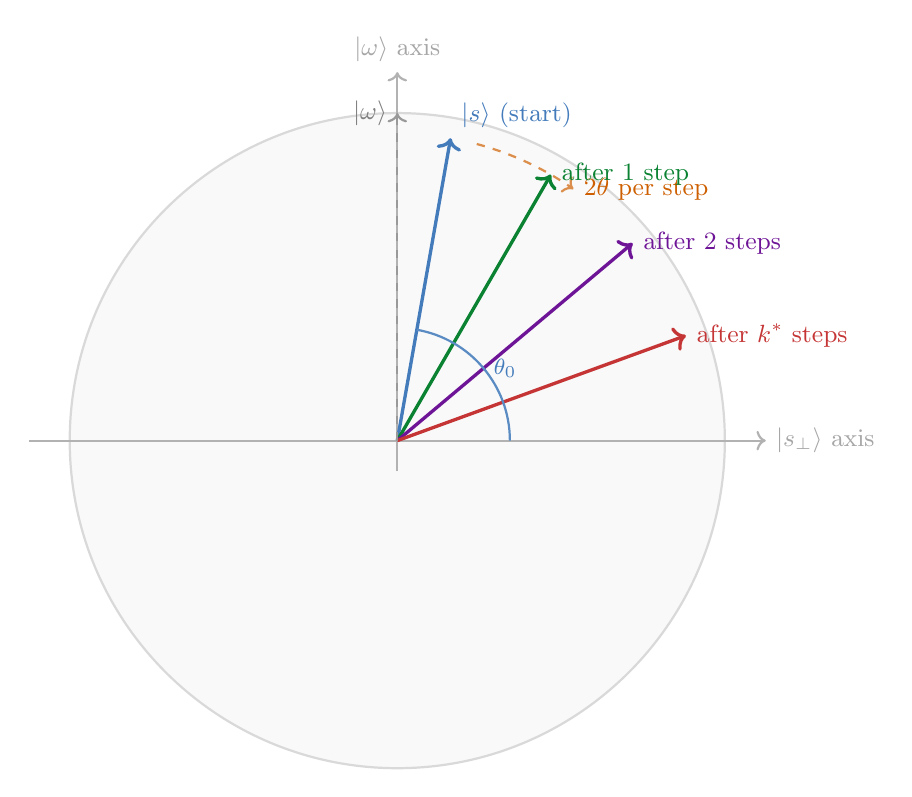
\begin{tikzpicture}[scale=1.3]
  \draw[thick,gray!30,fill=gray!5] (0,0) circle (3.2cm);
  % axes
  \draw[->,thick,gray!60] (-3.6,0)--(3.6,0) node[right,gray!70,font=\small]{$\ket{s_\perp}$ axis};
  \draw[->,thick,gray!60] (0,-0.3)--(0,3.6) node[above,gray!70,font=\small]{$\ket{\omega}$ axis};
  % arc indicating rotation
  \draw[->,thick,qorange!70,dashed] ({3.0*cos(75)},{3.0*sin(75)})
        arc[start angle=75,end angle=55,radius=3.0]
        node[right,qorange,font=\small]{$2\theta$ per step};
  % state vectors
  \foreach \ang/\col/\lab/\pos in {
      80/qblue!80/{$\ket{s}$ (start)}/above right,
      60/qgreen/{after 1 step}/right,
      40/qpurple/{after 2 steps}/right,
      20/qred!90/{after $k^*$ steps}/right}{
    \draw[->,very thick,\col] (0,0)--({3.0*cos(\ang)},{3.0*sin(\ang)})
      node[\pos,\col,font=\small]{\lab};
  }
  % target
  \draw[->,thick,black!40,dashed] (0,0)--(0,3.2) node[left,font=\small,black!50]{$\ket{\omega}$};
  % theta label
  \draw[qblue!70,thick] (1.1,0) arc[start angle=0,end angle=80,radius=1.1]
    node[midway,right,qblue!80,font=\footnotesize]{$\theta_0$};
\end{tikzpicture}

\vspace{1.2cm}
{\normalsize\textbf{Prerequisites:} Quantum states, Dirac notation, single- and multi-qubit gates,}\\
{\normalsize tensor products, measurement postulate.}\\[0.5cm]
{\normalsize\textbf{Goals:} Understand the oracle model; derive the Grover iterate geometrically}\\
{\normalsize and algebraically; prove the $\Order{\sqrt{N}}$ speedup; work through complete examples.}\\[1.5cm]
{\color{qblue}\rule{\linewidth}{1pt}}
\end{titlepage}

\tableofcontents
\newpage

%% ===========================================================
\section{Motivation: Why Quantum Search?}
\label{sec:motivation}

\subsection{The Classical Unordered Search Problem}

Suppose you have a list of $N$ items in \emph{no particular order}. You are given a black-box function that can check whether a given item is the one you seek. How many checks do you need?

\begin{itemize}
  \item \textbf{Best case:} 1 (you get lucky on the first try).
  \item \textbf{Worst case:} $N$ (the target is the last item checked).
  \item \textbf{Average case:} $N/2$.
\end{itemize}

Without any structure in the data (no sorting, no hash table), there is \emph{no classical shortcut}. The lower bound is provably $\Omega(N)$.

\subsection{The Quantum Advantage}

Quantum mechanics allows us to query all $N$ items \emph{simultaneously} via superposition, and then use \textbf{amplitude amplification} to make the target item stand out. The result, due to Lov Grover (1996), is:

\begin{thmbox}{Grover's Main Result}
An unordered database of $N$ items can be searched using $\Order{\sqrt{N}}$ quantum queries. This is a \textbf{quadratic speedup} over the classical $\Order{N}$, and it is \textbf{provably optimal} — no quantum algorithm can do better.
\end{thmbox}

\begin{notebox}
A quadratic speedup may sound modest, but it is enormous in practice. For $N = 10^{12}$ (one trillion items), classical search needs $\sim 10^{12}$ steps, while Grover needs only $\sim 10^6$ steps — a \emph{million-fold} reduction.
\end{notebox}

%% ===========================================================
\section{Problem Setup and Oracle Model}
\label{sec:setup}

\subsection{Formal Problem Statement}

\begin{defbox}{Unstructured Search}
Let $n \in \mathbb{N}$ and $N = 2^n$. We are given a function
\[
  f : \{0,1\}^n \longrightarrow \{0,1\}
\]
implemented as a quantum oracle (black box). There exists a unique \textbf{target} $\omega \in \{0,1\}^n$ such that
\[
  f(x) = \begin{cases} 1 & \text{if } x = \omega \\ 0 & \text{if } x \neq \omega \end{cases}
\]
\textbf{Goal:} find $\omega$ by querying $f$ as few times as possible.
\end{defbox}

We work in the $n$-qubit Hilbert space $\mathcal{H} = (\mathbb{C}^2)^{\otimes n}$ with the computational basis $\{\ket{x} : x \in \{0,1\}^n\}$, so $\dim \mathcal{H} = N$.

\subsection{The Standard Oracle}

The standard reversible oracle is a unitary on $n+1$ qubits:
\[
  O_f : \ket{x}\ket{b} \;\longmapsto\; \ket{x}\ket{b \oplus f(x)}, \qquad x \in \{0,1\}^n,\; b \in \{0,1\}
\]

The top $n$ qubits are the \textbf{query register}; the bottom qubit is the \textbf{target/ancilla register}.

\subsection{The Phase Oracle via Kick-Back}
\label{ssec:phasekickback}

We derive the \textbf{phase oracle} from $O_f$ by the \emph{phase kick-back trick}. Initialise the ancilla in $\ket{-} = \tfrac{1}{\sqrt{2}}(\ket{0}-\ket{1})$:

\begin{align}
  O_f\ket{x}\ket{-}
  &= O_f\ket{x}\,\tfrac{1}{\sqrt{2}}\bigl(\ket{0}-\ket{1}\bigr) \notag\\
  &= \tfrac{1}{\sqrt{2}}\bigl(\ket{x}\ket{f(x)} - \ket{x}\ket{1\oplus f(x)}\bigr) \notag\\
  &= \tfrac{1}{\sqrt{2}}\ket{x}\bigl(\ket{f(x)}-\ket{1\oplus f(x)}\bigr) \notag\\[4pt]
  &= (-1)^{f(x)}\ket{x}\ket{-} \label{eq:kickback}
\end{align}

Since the ancilla is unchanged, we can ignore it and define the \textbf{phase oracle} acting on $n$ qubits:

\begin{defbox}{Phase Oracle $U_f$}
\[
  U_f\ket{x} = (-1)^{f(x)}\ket{x} =
  \begin{cases}
    -\ket{x} & \text{if } x = \omega\\
    \phantom{-}\ket{x} & \text{if } x \neq \omega
  \end{cases}
\]
Equivalently, as an outer-product formula:
\[
  \boxed{U_f = I - 2\proj{\omega}}
\]
\end{defbox}

\textbf{Verification:}
\[
  (I - 2\proj{\omega})\ket{x} = \ket{x} - 2\underbrace{\ip{\omega}{x}}_{=\delta_{x\omega}}\ket{\omega}
  = \begin{cases} -\ket{\omega} & x=\omega\\ \ket{x} & x\neq\omega \end{cases}\checkmark
\]

\subsection{Oracle Circuit Diagram}

\begin{figure}[H]
\centering
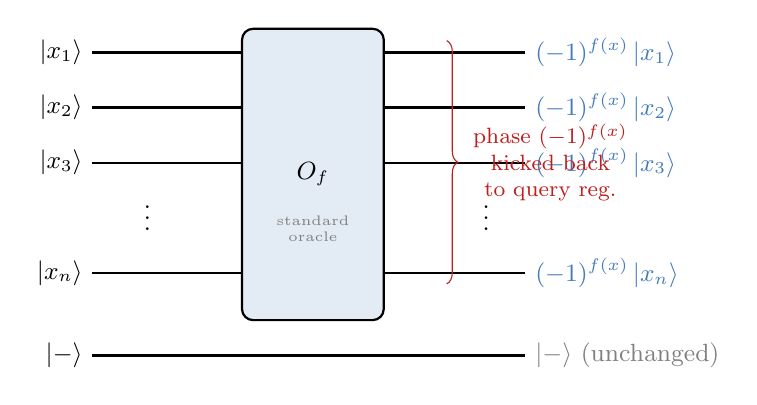
\begin{tikzpicture}[>=Stealth,font=\small,
    gate/.style={draw,fill=qblue!18,minimum width=1.6cm,minimum height=0.7cm,
                 rounded corners=2pt,font=\small}]
  \def\sep{0.7}   % vertical sep between wires
  \def\gx{2.8}    % x position of gate

  % Wires and labels — query register
  \foreach \i/\lab in {0/$\ket{x_1}$,1/$\ket{x_2}$,2/$\ket{x_3}$}{
    \pgfmathsetmacro{\y}{-\i*\sep}
    \draw[thick] (0,\y) -- (5.5,\y);
    \node[left] at (0,\y) {\lab};
    \node[right,qblue!80] at (5.5,\y) {$(-1)^{f(x)}\ket{x_{\the\numexpr\i+1\relax}}\vphantom{(-1)}$};
  }
  % dots
  \node at (0.7,-3*\sep+0.1) {$\vdots$};
  \node at (5.0,-3*\sep+0.1) {$\vdots$};

  % n-th wire
  \pgfmathsetmacro{\yn}{-4*\sep}
  \draw[thick] (0,\yn) -- (5.5,\yn);
  \node[left] at (0,\yn) {$\ket{x_n}$};
  \node[right,qblue!80] at (5.5,\yn) {$(-1)^{f(x)}\ket{x_n}\vphantom{(-1)}$};

  % ancilla wire
  \pgfmathsetmacro{\ya}{-5.5*\sep}
  \draw[thick] (0,\ya) -- (5.5,\ya);
  \node[left] at (0,\ya) {$\ket{-}$};
  \node[right,gray] at (5.5,\ya) {$\ket{-}$ (unchanged)};

  % Big oracle box spanning query + ancilla
  \draw[thick,fill=qblue!12,rounded corners=4pt]
    (\gx-0.9, {-4.5*\sep-0.25}) rectangle (\gx+0.9, {0.3});
  \node[font=\bfseries\small,align=center] at (\gx, {-2.2*\sep}) {$O_f$};
  \node[font=\tiny,align=center,gray] at (\gx, {-3.2*\sep}) {standard\\oracle};

  % Brace: phase kick-back effect
  \draw[decorate,decoration={brace,amplitude=4pt},qred]
    (4.5,0.15) -- (4.5,{-4.2*\sep})
    node[midway,right=6pt,qred,font=\footnotesize,align=center]
      {phase $(-1)^{f(x)}$\\kicked back\\to query reg.};
\end{tikzpicture}
\caption{Standard oracle $O_f$ with ancilla $\ket{-}$. The phase $(-1)^{f(x)}$ is ``kicked back'' onto the query register, leaving the ancilla unchanged. This implements the phase oracle $U_f$.}
\label{fig:oracle}
\end{figure}

%% ===========================================================
\section{Initial State and Key Operators}
\label{sec:operators}

\subsection{Uniform Superposition}

Apply the $n$-qubit Hadamard transform $H^{\otimes n}$ to $\ket{0}^{\otimes n}$:
\[
  \HH\ket{0}^{\otimes n}
  = \underbrace{\frac{1}{\sqrt{N}}\sum_{x=0}^{N-1}\ket{x}}_{\displaystyle\ket{s}}
\]

Every basis state has equal amplitude $1/\sqrt{N}$. Key inner products:
\[
  \ip{s}{\omega} = \frac{1}{\sqrt{N}}, \qquad
  \ip{s}{s} = 1, \qquad
  \ip{\omega}{\omega} = 1.
\]

\subsection{The Two Grover Operations}

\subsubsection{Operation 1 — Oracle: Reflect about $\ket{\omega}^\perp$}

\[
  \boxed{U_f = I - 2\proj{\omega}}
\]

Geometrically: $U_f$ is a \textbf{reflection of the state vector about the hyperplane perpendicular to $\ket{\omega}$}. It flips the sign of the $\ket{\omega}$ component and leaves everything orthogonal to $\ket{\omega}$ unchanged.

\subsubsection{Operation 2 — Diffusion: Reflect about $\ket{s}$}

\[
  \boxed{D = 2\proj{s} - I}
\]

In the computational basis, $D$ can be implemented as $D = \HH(2\proj{0}-I)\HH$, which gives:

\begin{align}
  D\ket{x} &= (2\proj{s}-I)\ket{x}
            = 2\ip{s}{x}\ket{s} - \ket{x}
            = \frac{2}{N}\sum_{y}\ket{y} - \ket{x}
\end{align}

If the current state is $\ket{\psi} = \sum_x \alpha_x\ket{x}$, then after $D$:
\[
  \alpha_x \;\longmapsto\; 2\bar{\alpha} - \alpha_x,
  \qquad \bar{\alpha} = \frac{1}{N}\sum_{x=0}^{N-1}\alpha_x
\]

\begin{keybox}{Inversion About the Mean}
The diffusion operator $D$ performs \textbf{inversion about the mean}: each amplitude is reflected around the average amplitude $\bar\alpha$.
\begin{itemize}
  \item If $\alpha_x < \bar\alpha$: the amplitude \emph{increases}.
  \item If $\alpha_x > \bar\alpha$: the amplitude \emph{decreases}.
\end{itemize}
After the oracle flips the target's amplitude to $-|\alpha_\omega|$, the target amplitude is far below the mean. Inversion about the mean then pushes it significantly upward.
\end{keybox}

\subsection{The Grover Iterate}

\begin{defbox}{Grover Iterate $G$}
\[
  G = D \cdot U_f = (2\proj{s}-I)(I-2\proj{\omega})
\]
One application of $G$ is called a \textbf{Grover step} or \textbf{Grover iterate}.
\end{defbox}

\subsection{Circuit Diagrams for $U_f$ and $D$}

\begin{figure}[H]
\centering
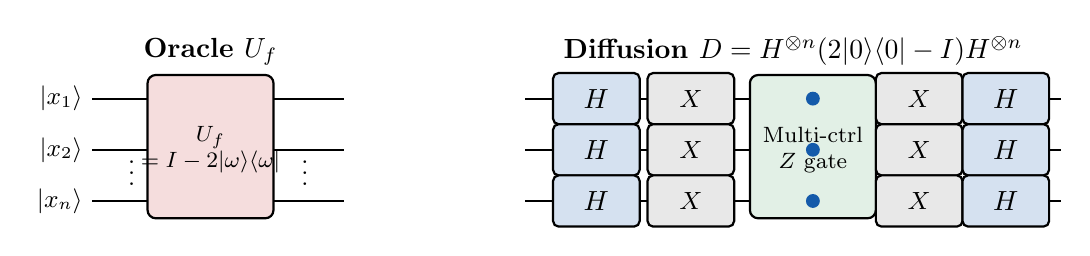
\begin{tikzpicture}[>=Stealth,font=\small,
    gate/.style={draw,thick,fill=#1!18,minimum width=1.1cm,minimum height=0.65cm,
                 rounded corners=2pt}]
  % ---- Oracle U_f ----
  \node[font=\bfseries] at (1.5,0.6) {Oracle $U_f$};
  \foreach \i/\lab in {0/1,1/2,2/n}{
    \pgfmathsetmacro{\y}{-\i*0.65}
    \draw[thick] (0,\y) -- (3.2,\y);
    \node[left,font=\small] at (0,\y) {$\ket{x_{\lab}}$};
  }
  \node[font=\small] at (0.5,-1.3*0.65) {$\vdots$};
  \node[font=\small] at (2.7,-1.3*0.65) {$\vdots$};
  \draw[thick,fill=qred!15,rounded corners=3pt]
    (0.7,-2*0.65-0.22) rectangle (2.3,0.3);
  \node[font=\bfseries\footnotesize,align=center] at (1.5,-0.65) {$U_f$\\$=I-2\proj{\omega}$};

  % ---- Diffusion D ----
  \begin{scope}[xshift=5.5cm]
  \node[font=\bfseries] at (3.4,0.6) {Diffusion $D = H^{\otimes n}(2\proj{0}-I)H^{\otimes n}$};
  \foreach \i in {0,1,2}{
    \pgfmathsetmacro{\y}{-\i*0.65}
    \draw[thick] (0,\y) -- (6.8,\y);
  }
  \node[font=\small] at (0.5,-1.3*0.65) {$\vdots$};
  \node[font=\small] at (6.3,-1.3*0.65) {$\vdots$};
  % H gates left
  \foreach \i in {0,1,2}{
    \pgfmathsetmacro{\y}{-\i*0.65}
    \node[gate=qblue,font=\bfseries] at (0.9,\y) {$H$};
  }
  % X gates
  \foreach \i in {0,1,2}{
    \pgfmathsetmacro{\y}{-\i*0.65}
    \node[gate=gray] at (2.1,\y) {$X$};
  }
  % Multi-controlled Z box
  \draw[thick,fill=qgreen!12,rounded corners=3pt]
    (2.85,-2*0.65-0.22) rectangle (4.45,0.3);
  \node[font=\footnotesize,align=center] at (3.65,-0.65)
    {Multi-ctrl\\$Z$ gate};
  % dots in ctrl box
  \foreach \i in {0,1,2}{
    \pgfmathsetmacro{\y}{-\i*0.65}
    \fill[qblue] (3.65,\y) circle (2.5pt);
  }
  % X gates right
  \foreach \i in {0,1,2}{
    \pgfmathsetmacro{\y}{-\i*0.65}
    \node[gate=gray] at (5.0,\y) {$X$};
  }
  % H gates right
  \foreach \i in {0,1,2}{
    \pgfmathsetmacro{\y}{-\i*0.65}
    \node[gate=qblue,font=\bfseries] at (6.1,\y) {$H$};
  }
  \end{scope}
\end{tikzpicture}
\caption{Left: phase oracle $U_f$. Right: decomposition of the diffusion operator $D$. The $(2\proj{0}-I)$ operation is a phase flip on $\ket{0\cdots0}$, implemented with $X$ gates and a multi-controlled-$Z$ (equivalently, multi-controlled-$X$ with a phase kickback ancilla).}
\label{fig:circuits}
\end{figure}

\begin{figure}[H]
\centering
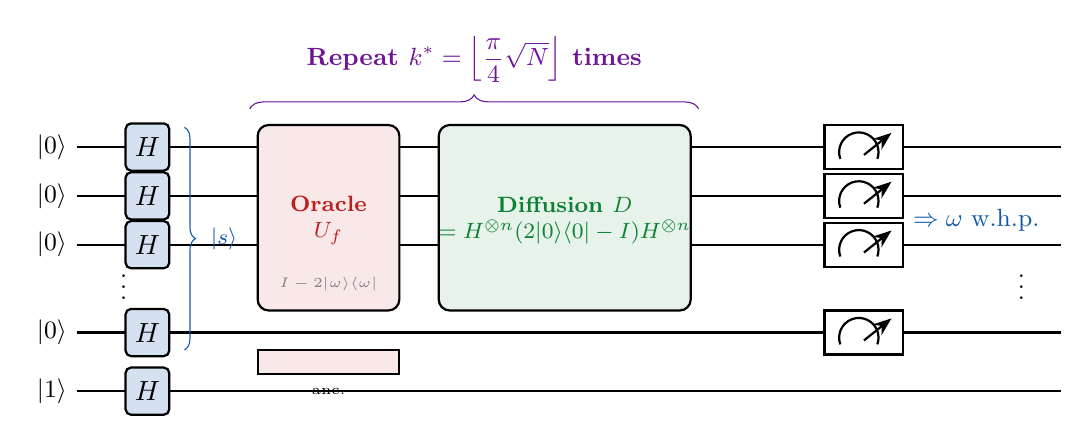
\begin{tikzpicture}[>=Stealth,font=\small,
    gate/.style={draw,thick,fill=#1!18,minimum width=1.0cm,minimum height=0.6cm,
                 rounded corners=2pt}]
  % Full Grover circuit — n data qubits + 1 ancilla
  \def\wsep{0.62}
  \def\n{3}   % draw 3 data qubits + dots

  % ── wires ──
  \foreach \i in {0,1,2}{
    \pgfmathsetmacro{\y}{-\i*\wsep}
    \draw[thick] (0,\y) -- (12.5,\y);
    \node[left] at (0,\y) {$\ket{0}$};
  }
  \node at (0.6,-2.7*\wsep) {$\vdots$};
  \node at (12.0,-2.7*\wsep) {$\vdots$};
  \pgfmathsetmacro{\ynq}{-3.8*\wsep}
  \draw[thick] (0,\ynq) -- (12.5,\ynq);
  \node[left] at (0,\ynq) {$\ket{0}$};
  % ancilla
  \pgfmathsetmacro{\yanc}{-5.0*\wsep}
  \draw[thick] (0,\yanc) -- (12.5,\yanc);
  \node[left] at (0,\yanc) {$\ket{1}$};

  % ── Initial H on each data qubit ──
  \foreach \i in {0,1,2}{
    \pgfmathsetmacro{\y}{-\i*\wsep}
    \node[gate=qblue,font=\bfseries,minimum width=0.55cm] at (0.9,\y) {$H$};
  }
  \node[gate=qblue,font=\bfseries,minimum width=0.55cm] at (0.9,\ynq) {$H$};
  % H on ancilla to make |->
  \node[gate=qblue,font=\bfseries,minimum width=0.55cm] at (0.9,\yanc) {$H$};

  % Brace: "prepare |s>" 
  \draw[decorate,decoration={brace,amplitude=4pt,raise=2pt},qblue]
    (1.3,0.25) -- (1.3,{\ynq-0.22})
    node[midway,right=8pt,qblue,font=\footnotesize]{$\ket{s}$};

  % ── Grover iterate box (repeated k* times) ──
  % Oracle box
  \draw[thick,fill=qred!10,rounded corners=4pt]
    (2.3,{\ynq+0.28}) rectangle (4.1,{0.28});
  \node[font=\bfseries\footnotesize,align=center,qred] at (3.2,{-1.5*\wsep}) {Oracle\\$U_f$};
  \node[font=\tiny,gray] at (3.2,{-2.8*\wsep}) {$I-2\proj{\omega}$};
  % connect ancilla to oracle box
  \draw[thick,fill=qred!10] (2.3,{\yanc+0.22}) rectangle (4.1,{\ynq-0.22});
  \node[font=\tiny,align=center] at (3.2,\yanc) {anc.};

  % Diffusion box
  \draw[thick,fill=qgreen!10,rounded corners=4pt]
    (4.6,{\ynq+0.28}) rectangle (7.8,{0.28});
  \node[font=\bfseries\footnotesize,align=center,qgreen] at (6.2,{-1.5*\wsep})
    {Diffusion $D$\\$=H^{\otimes n}(2\proj{0}-I)H^{\otimes n}$};

  % "Repeat k* times" brace
  \draw[decorate,decoration={brace,amplitude=5pt,raise=3pt},qpurple]
    (2.2,0.38) -- (7.9,0.38)
    node[midway,above=9pt,qpurple,font=\small\bfseries]{Repeat $k^*=\left\lfloor\dfrac{\pi}{4}\sqrt{N}\right\rfloor$ times};

  % ── measure ──
  \foreach \i in {0,1,2}{
    \pgfmathsetmacro{\y}{-\i*\wsep}
    % meter symbol
    \draw[thick,fill=white] (9.5,{\y-0.28}) rectangle (10.5,{\y+0.28});
    \draw[thick] (9.7,{\y-0.15}) arc[start angle=200,end angle=-20,radius=0.25];
    \draw[->,thick] (10.0,{\y-0.1}) -- (10.35,{\y+0.18});
  }
  \draw[thick,fill=white] (9.5,{\ynq-0.28}) rectangle (10.5,{\ynq+0.28});
  \draw[thick] (9.7,{\ynq-0.15}) arc[start angle=200,end angle=-20,radius=0.25];
  \draw[->,thick] (10.0,{\ynq-0.1}) -- (10.35,{\ynq+0.18});

  % output label
  \node[right,qblue,font=\small] at (10.5,{-1.5*\wsep}) {$\Rightarrow\omega$ w.h.p.};
\end{tikzpicture}
\caption{Full Grover circuit. The Grover iterate $G = D\cdot U_f$ is applied $k^* = \lfloor\frac{\pi}{4}\sqrt{N}\rfloor$ times. Final measurement of the data register yields the target $\omega$ with probability close to 1.}
\label{fig:full_circuit}
\end{figure}

%% ===========================================================
\section{Geometric Analysis}
\label{sec:geometry}

This section gives the cleanest and most intuitive explanation of Grover's algorithm. The key insight is that the entire $N$-dimensional evolution can be understood as rotation in a \textbf{2-dimensional plane}.

\subsection{The 2D Invariant Subspace}

Define two orthonormal-in-span vectors:
\begin{align}
  \ket{\omega} &\quad \text{(the target state)} \\[4pt]
  \ket{s'} &= \frac{1}{\sqrt{N-1}}\sum_{x \neq \omega}\ket{x}
              \quad\text{(uniform superposition over non-targets)}
\end{align}

Note $\ip{s'}{\omega} = 0$. We can write the initial state $\ket{s}$ as:
\[
  \ket{s} = \underbrace{\frac{1}{\sqrt{N}}}_{\sin\theta}\ket{\omega}
           + \underbrace{\sqrt{\frac{N-1}{N}}}_{\cos\theta}\ket{s'}
\]
where
\[
  \boxed{\sin\theta = \frac{1}{\sqrt{N}}, \qquad \theta = \arcsin\!\left(\frac{1}{\sqrt{N}}\right)}
\]

For large $N$: $\sin\theta \approx \theta \approx 1/\sqrt{N}$ (small angle).

\begin{thmbox}{Invariance of the 2D Plane}
Both $U_f$ and $D$ preserve the subspace $\mathcal{V} = \mathrm{span}\{\ket{\omega},\,\ket{s'}\}$.\\[4pt]
\textbf{Proof:} 
\begin{itemize}
  \item $U_f = I - 2\proj{\omega}$ maps $\ket{\omega}\mapsto-\ket{\omega}$ and $\ket{s'}\mapsto\ket{s'}$, so $\mathcal{V}$ is preserved.
  \item $D = 2\proj{s}-I$: since $\ket{s}\in\mathcal{V}$, $D$ maps any vector in $\mathcal{V}$ to a vector in $\mathcal{V}$.\quad$\square$
\end{itemize}
\end{thmbox}

\subsection{What $U_f$ Does Geometrically}

In the 2D picture with horizontal axis $\ket{s'}$ and vertical axis $\ket{\omega}$:

$U_f = I - 2\proj{\omega}$ \textbf{reflects} the state vector about the horizontal axis $\ket{s'}$ (it negates the $\ket{\omega}$ component).

\begin{figure}[H]
\centering
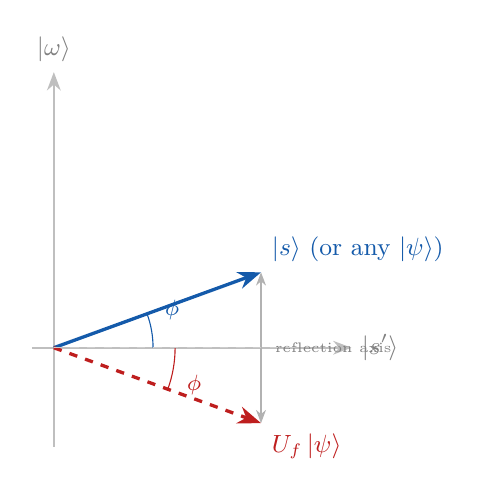
\begin{tikzpicture}[>=Stealth,scale=2.8]
  % axes
  \draw[->,thick,gray!50] (-0.1,0)--(1.35,0) node[right,gray,font=\small]{$\ket{s'}$};
  \draw[->,thick,gray!50] (0,-0.45)--(0,1.25) node[above,gray,font=\small]{$\ket{\omega}$};

  % angle value
  \def\th{20}

  % initial state s at angle theta above horizontal
  \draw[->,very thick,qblue]
    (0,0)--({cos(\th)},{sin(\th)})
    node[above right,qblue,font=\small]{$\ket{s}$ (or any $\ket{\psi}$)};

  % after oracle: reflect about horizontal => negate omega component
  \draw[->,very thick,qred,dashed]
    (0,0)--({cos(\th)},{-sin(\th)})
    node[below right,qred,font=\small]{$U_f\ket{\psi}$};

  % reflection indicator
  \draw[<->,thin,gray!60] ({cos(\th)},{sin(\th)})--({cos(\th)},{-sin(\th)});
  \node[right,gray,font=\tiny] at ({cos(\th)+0.02},0){reflection axis};

  % Angle annotation above
  \draw[qblue,thin] (0.45,0) arc[start angle=0,end angle=\th,radius=0.45];
  \node[right,qblue,font=\footnotesize] at (0.46,{0.5*sin(\th)}){$\phi$};

  % Angle annotation below
  \draw[qred,thin] (0.55,0) arc[start angle=0,end angle=-\th,radius=0.55];
  \node[right,qred,font=\footnotesize] at (0.56,{-0.5*sin(\th)}){$\phi$};

  % Horizontal dashed line
  \draw[dashed,gray!40] (0,0)--(1.1,0);
\end{tikzpicture}
\caption{$U_f$ reflects the state vector about the $\ket{s'}$ axis (horizontal). The angle below the horizontal equals the angle above. The $\ket{\omega}$ component changes sign.}
\label{fig:uf_geometry}
\end{figure}

\subsection{What $D$ Does Geometrically}

$D = 2\proj{s}-I$ \textbf{reflects} the state vector about the $\ket{s}$ axis.

\begin{figure}[H]
\centering
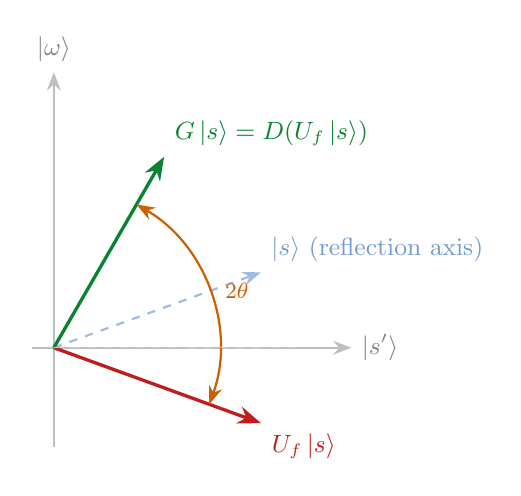
\begin{tikzpicture}[>=Stealth,scale=2.8]
  \draw[->,thick,gray!50] (-0.1,0)--(1.35,0) node[right,gray,font=\small]{$\ket{s'}$};
  \draw[->,thick,gray!50] (0,-0.45)--(0,1.25) node[above,gray,font=\small]{$\ket{\omega}$};

  \def\th{20}   % theta
  \def\phi{-\th} % angle of input after oracle

  % s direction (dashed, reference axis)
  \draw[->,thick,qblue!40,dashed]
    (0,0)--({cos(\th)},{sin(\th)})
    node[above right,qblue!60,font=\small]{$\ket{s}$ (reflection axis)};

  % State input to D: at angle -theta (below horizontal)
  \draw[->,very thick,qred]
    (0,0)--({cos(\th)},{-sin(\th)})
    node[below right,qred,font=\small]{$U_f\ket{s}$};

  % After D: reflect about s-axis at angle +theta
  % reflection of -theta about theta gives 3*theta
  \draw[->,very thick,qgreen]
    (0,0)--({cos(3*\th)},{sin(3*\th)})
    node[above right,qgreen,font=\small]{$G\ket{s} = D(U_f\ket{s})$};

  % Arc showing 2*theta rotation
  \draw[<->,thin,qorange,thick]
    ({0.75*cos(-\th)},{0.75*sin(-\th)})
    arc[start angle=-\th,end angle=3*\th,radius=0.75]
    node[midway,right=2pt,qorange,font=\footnotesize]{$2\theta$};

  \draw[dashed,gray!40] (0,0)--(1.1,0);
\end{tikzpicture}
\caption{After $U_f$ rotates to angle $-\theta$, the diffusion $D$ reflects about $\ket{s}$ (at angle $+\theta$), bringing the state to angle $+3\theta$. Net rotation: $\theta \to 3\theta$, an increase of $2\theta$.}
\label{fig:d_geometry}
\end{figure}

\subsection{Full Grover Iterate: Rotation by $2\theta$}

\begin{thmbox}{Rotation Theorem}
Starting from a state at angle $\phi$ from $\ket{s'}$ (i.e., $\ket{\psi}=\sin\phi\,\ket{\omega}+\cos\phi\,\ket{s'}$), one application of $G = D\cdot U_f$ produces:
\[
  G\ket{\psi} = \sin(\phi+2\theta)\,\ket{\omega} + \cos(\phi+2\theta)\,\ket{s'}
\]
The state rotates by exactly $2\theta$ toward $\ket{\omega}$ in the $\{\ket{\omega},\ket{s'}\}$ plane.
\end{thmbox}

\textbf{Proof.}
\begin{enumerate}
  \item Start: $\ket{\psi} = \sin\phi\,\ket{\omega} + \cos\phi\,\ket{s'}$. Angle from $\ket{s'}$ is $\phi$.
  \item After $U_f$ (reflect about $\ket{s'}$): negate $\ket{\omega}$ component:
  \[
    U_f\ket{\psi} = -\sin\phi\,\ket{\omega} + \cos\phi\,\ket{s'}. \quad\text{Angle: }-\phi.
  \]
  \item After $D$ (reflect about $\ket{s}$ at angle $\theta$): a reflection of angle $-\phi$ about the line at angle $\theta$ gives angle $2\theta-(-\phi) = 2\theta+\phi$.
  \[
    G\ket{\psi} = \sin(2\theta+\phi)\,\ket{\omega} + \cos(2\theta+\phi)\,\ket{s'}.\quad\square
  \]
\end{enumerate}

\subsection{State After $k$ Iterations}

Starting from $\ket{s}$ at initial angle $\theta$:
\[
  \boxed{G^k\ket{s} = \sin\!\bigl((2k+1)\theta\bigr)\ket{\omega} + \cos\!\bigl((2k+1)\theta\bigr)\ket{s'}}
\]

\subsection{Optimal Number of Iterations}

Success probability after $k$ steps:
\[
  P_{\text{success}}(k) = \sin^2\!\bigl((2k+1)\theta\bigr)
\]
This is maximised when $(2k+1)\theta \approx \pi/2$, i.e.,
\[
  k^* = \left\lfloor\frac{\pi/2 - \theta}{2\theta}\right\rfloor
       = \left\lfloor\frac{\pi}{4\theta} - \frac{1}{2}\right\rfloor
       \approx \left\lfloor\frac{\pi}{4}\sqrt{N}\right\rfloor
\]
(using $\theta \approx 1/\sqrt{N}$ for large $N$).

\begin{figure}[H]
\centering
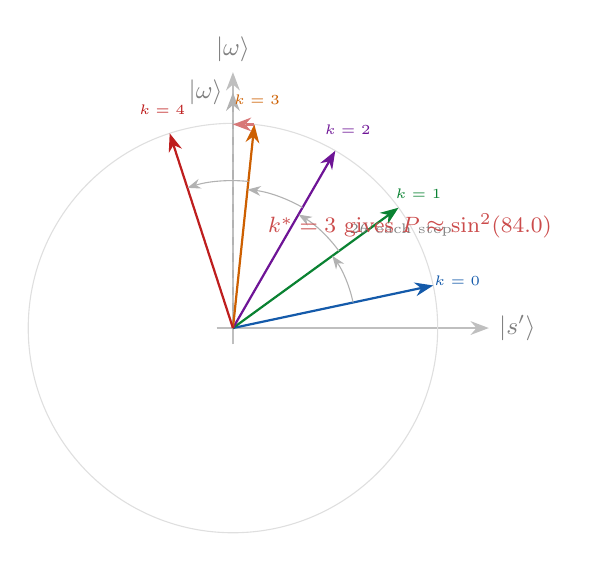
\begin{tikzpicture}[>=Stealth,scale=2.6]
  \draw[->,thick,gray!50] (-0.08,0)--(1.25,0) node[right,gray,font=\small]{$\ket{s'}$};
  \draw[->,thick,gray!50] (0,-0.08)--(0,1.25) node[above,gray,font=\small]{$\ket{\omega}$};
  \draw[thin,gray!25] (0,0) circle (1.0);

  \def\th{12}

  % Target
  \draw[->,thick,black!30,dashed] (0,0)--(0,1.15) node[left,black!50,font=\small]{$\ket\omega$};

  % State vectors at each k
  \foreach \k/\col in {0/qblue,1/qgreen,2/qpurple,3/qorange,4/qred}{
    \pgfmathsetmacro{\ang}{(2*\k+1)*\th}
    \draw[->,thick,\col] (0,0)--({cos(\ang)},{sin(\ang)});
    \node[\col,font=\tiny] at ({1.12*cos(\ang)},{1.12*sin(\ang)}) {$k=\k$};
  }

  % Rotation arcs between consecutive states
  \foreach \k in {0,1,2,3}{
    \pgfmathsetmacro{\a}{(2*\k+1)*\th}
    \pgfmathsetmacro{\b}{(2*\k+3)*\th}
    \pgfmathsetmacro{\r}{0.6+\k*0.04}
    \draw[->,thin,gray!60] ({\r*cos(\a)},{\r*sin(\a)})
      arc[start angle=\a,end angle=\b,radius=\r];
  }
  \node[gray,font=\tiny] at (0.82,0.48) {$2\theta$ each step};

  % k* annotation
  \pgfmathsetmacro{\kstar}{int(round(90/(2*\th)-0.5))}
  \pgfmathsetmacro{\angstar}{(2*\kstar+1)*\th}
  \draw[qred!60,thick,dashed,->] ({cos(\angstar)},{sin(\angstar)})--(0,{sin(\angstar)});
  \node[right,qred!80,font=\footnotesize] at ({cos(\angstar)+0.02},{sin(\angstar)*0.5})
    {$k^*=\kstar$ gives $P\approx\sin^2(\angstar°)$};
\end{tikzpicture}
\caption{Geometric view: the state rotates by $2\theta$ per Grover iterate, spiralling toward $\ket{\omega}$. The optimal stopping point $k^*$ is when the angle reaches $\approx90°$ from $\ket{s'}$.}
\label{fig:rotation_spiral}
\end{figure}

%% ===========================================================
\section{Algebraic Analysis}
\label{sec:algebra}

We now derive the same results purely algebraically and explicitly connect to the geometric picture.

\subsection{Amplitude Recurrence}

Write the state after $k$ iterates as:
\[
  \ket{\psi_k} = \alpha_k\ket{\omega} + \beta_k\sum_{x\neq\omega}\ket{x}
\]
(by symmetry, all non-target amplitudes remain equal throughout).

\textbf{Initial values:} $\alpha_0 = \beta_0 = 1/\sqrt{N}$.

\subsubsection*{Step A: Apply $U_f$}

\[
  U_f\ket{\psi_k} = -\alpha_k\ket{\omega} + \beta_k\sum_{x\neq\omega}\ket{x}
\]

\subsubsection*{Step B: Compute Mean Before Diffusion}

\[
  \bar{\mu} = \frac{-\alpha_k + (N-1)\beta_k}{N}
\]

\subsubsection*{Step C: Apply $D$ (Inversion About Mean)}

\begin{align}
  \alpha_{k+1} &= 2\bar{\mu} - (-\alpha_k)
    = 2\bar\mu + \alpha_k
    = \frac{-2\alpha_k+2(N-1)\beta_k}{N}+\alpha_k
    = \frac{(N-2)\alpha_k + 2(N-1)\beta_k}{N} \label{eq:rec1}\\[6pt]
  \beta_{k+1}  &= 2\bar{\mu} - \beta_k
    = \frac{-2\alpha_k+2(N-1)\beta_k}{N}-\beta_k
    = \frac{-2\alpha_k+(N-2)\beta_k}{N} \label{eq:rec2}
\end{align}

In matrix form:
\[
  \begin{pmatrix}\alpha_{k+1}\\\beta_{k+1}\end{pmatrix}
  = \underbrace{\frac{1}{N}\begin{pmatrix}N-2 & 2(N-1)\\-2 & N-2\end{pmatrix}}_{M}
  \begin{pmatrix}\alpha_k\\\beta_k\end{pmatrix}
\]

\subsection{Closed-Form Solution}

\begin{thmbox}{Amplitude Formula}
The exact solution to the recurrence with $\alpha_0=\beta_0=1/\sqrt{N}$ is:
\begin{align}
  \alpha_k &= \sin\!\bigl((2k+1)\theta\bigr) \label{eq:alpha_closed}\\[4pt]
  \beta_k  &= \frac{\cos\!\bigl((2k+1)\theta\bigr)}{\sqrt{N-1}} \label{eq:beta_closed}
\end{align}
where $\theta = \arcsin(1/\sqrt{N})$.
\end{thmbox}

\textbf{Verification:}
\begin{itemize}
  \item \textbf{Initial condition} ($k=0$): $\alpha_0 = \sin\theta = 1/\sqrt{N}$\,\checkmark \quad $\beta_0 = \cos\theta/\sqrt{N-1} = \sqrt{(N-1)/N}/\sqrt{N-1} = 1/\sqrt{N}$\,\checkmark
  \item \textbf{Normalisation}: $|\alpha_k|^2 + (N-1)|\beta_k|^2 = \sin^2((2k+1)\theta) + \cos^2((2k+1)\theta) = 1$\,\checkmark
  \item \textbf{Recurrence check (sketch)}: substituting into \eqref{eq:rec1} and using $\sin(A+2\theta) = \sin A\cos 2\theta + \cos A\sin 2\theta$ with $\cos 2\theta = 1-2/N$ and $\sin 2\theta = 2\sqrt{N-1}/N$ confirms the formula. $\square$
\end{itemize}

\subsection{Equivalence with the Geometric Picture}

The geometric result was:
\[
  G^k\ket{s} = \sin((2k+1)\theta)\ket{\omega} + \cos((2k+1)\theta)\ket{s'}
\]

Since $\ket{s'} = \frac{1}{\sqrt{N-1}}\sum_{x\neq\omega}\ket{x}$, the amplitude of each non-target state in the geometric formula is $\cos((2k+1)\theta)/\sqrt{N-1}$, which exactly matches the algebraic $\beta_k$ in \eqref{eq:beta_closed}. \\[4pt]
\textbf{The geometric picture is a faithful, lower-dimensional representation of the algebraic recurrence.}

\begin{center}
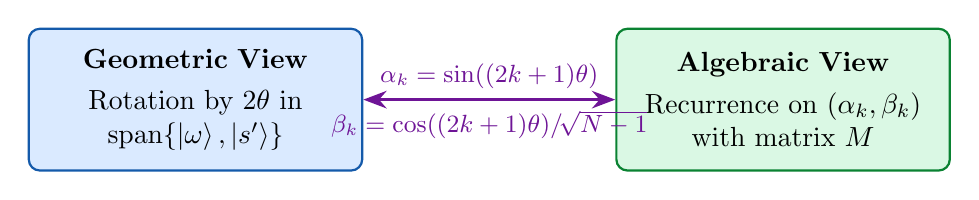
\begin{tikzpicture}[node distance=3.2cm,>=Stealth]
  \node[draw=qblue,fill=lightblue,rounded corners,thick,
        minimum width=4.2cm,minimum height=1.8cm,text width=4.0cm,align=center]
    (geo) {\textbf{Geometric View}\\[3pt]
           Rotation by $2\theta$ in\\$\mathrm{span}\{\ket\omega,\ket{s'}\}$};
  \node[draw=qgreen,fill=lightgreen,rounded corners,thick,
        minimum width=4.2cm,minimum height=1.8cm,text width=4.0cm,align=center,
        right=of geo]
    (alg) {\textbf{Algebraic View}\\[3pt]
           Recurrence on $(\alpha_k,\beta_k)$\\with matrix $M$};
  \draw[<->,very thick,qpurple] (geo)--(alg)
    node[midway,above,qpurple,font=\small]{$\alpha_k=\sin((2k+1)\theta)$}
    node[midway,below,qpurple,font=\small]{$\beta_k=\cos((2k+1)\theta)/\!\sqrt{N-1}$};
\end{tikzpicture}
\end{center}

%% ===========================================================
\section{Worked Examples}
\label{sec:examples}

\subsection{Example 1: $N=4$ ($n=2$ qubits), $\omega = 11$}

\textbf{Setup:} $N=4$, $\theta=\arcsin(1/2)=30°$, $k^*=\lfloor\frac\pi 4\cdot 2\rfloor=1$.

\medskip
\noindent\textbf{Initial state after $H^{\otimes 2}$:}
\[
  \ket{s} = \tfrac{1}{2}\ket{00}+\tfrac{1}{2}\ket{01}+\tfrac{1}{2}\ket{10}+\tfrac{1}{2}\ket{11}
\]

\noindent\textbf{After Oracle $U_f$ (flip sign of $\ket{11}$):}
\[
  \tfrac{1}{2}\ket{00}+\tfrac{1}{2}\ket{01}+\tfrac{1}{2}\ket{10}-\tfrac{1}{2}\ket{11}
\]

\noindent\textbf{Mean amplitude:}
\[
  \bar\alpha = \tfrac{1}{4}\!\left(\tfrac{1}{2}+\tfrac{1}{2}+\tfrac{1}{2}-\tfrac{1}{2}\right) = \tfrac{1}{4}
\]

\noindent\textbf{After Diffusion ($\alpha'_x = 2\bar\alpha - \alpha_x$):}
\begin{align*}
  \ket{00}&: 2\cdot\tfrac{1}{4}-\tfrac{1}{2} = 0 \\
  \ket{01}&: 2\cdot\tfrac{1}{4}-\tfrac{1}{2} = 0 \\
  \ket{10}&: 2\cdot\tfrac{1}{4}-\tfrac{1}{2} = 0 \\
  \ket{11}&: 2\cdot\tfrac{1}{4}-(-\tfrac{1}{2}) = \mathbf{1}
\end{align*}

\[
  \ket{\psi_1} = \ket{11} \quad\Rightarrow\quad P(\text{success}) = 1^2 = \mathbf{100\%}!
\]

\begin{figure}[H]
\centering
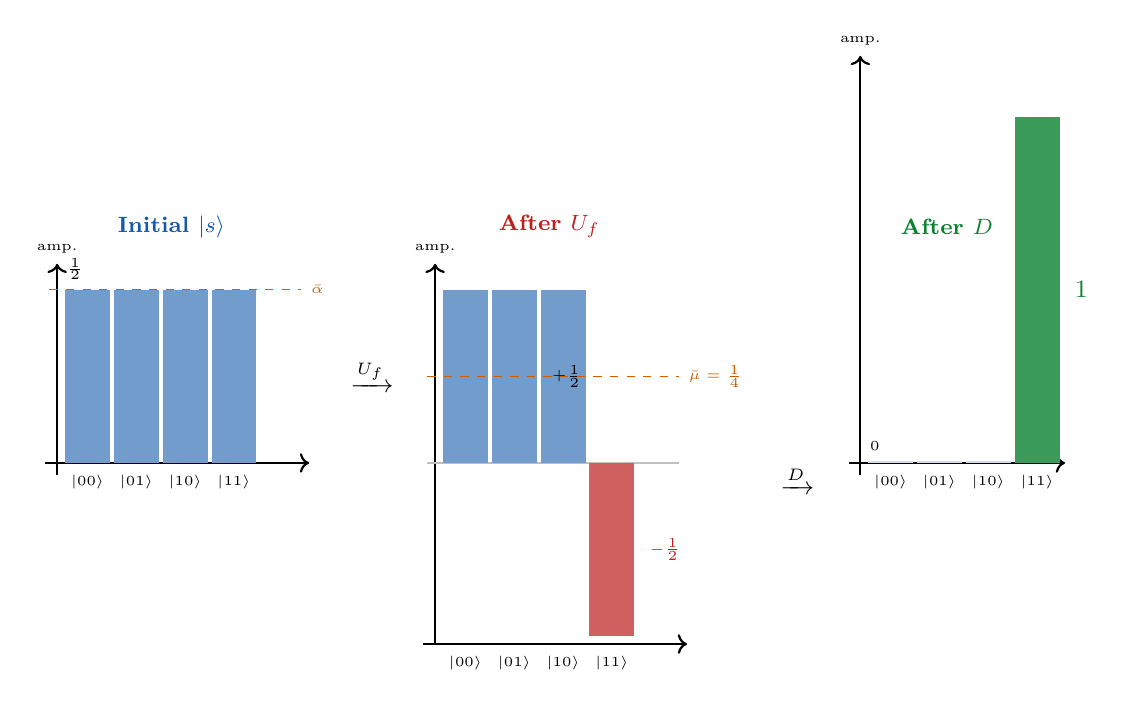
\begin{tikzpicture}[font=\small]
\def\bw{0.62}
\def\sc{2.2}   % scale: bar height for amplitude 0.5

% Panel A
\begin{scope}[xshift=0cm]
  \node[font=\footnotesize\bfseries,qblue] at (1.45,3.0) {Initial $\ket{s}$};
  \draw[->,thick] (-0.15,0)--(3.2,0);
  \draw[->,thick] (0,-0.15)--(0,{1.15*\sc}) node[above,font=\tiny]{amp.};
  \foreach \i/\lab in {0/00,1/01,2/10,3/11}{
    \fill[qblue!60] ({\bw*\i+0.1},0) rectangle ({\bw*\i+0.1+\bw-0.05},\sc);
    \node[font=\tiny,below=1pt] at ({\bw*\i+0.1+(\bw-0.05)/2},0) {$\ket{\lab}$};
  }
  \node[font=\tiny,above right=0pt] at (0,\sc) {$\tfrac{1}{2}$};
  \draw[dashed,qorange] (-0.1,\sc)--(3.1,\sc) node[right,font=\tiny,qorange]{$\bar\alpha$};
\end{scope}

% Arrow
\node at (4.0,{0.5*\sc}) {$\xrightarrow{U_f}$};

% Panel B: after oracle
\begin{scope}[xshift=4.8cm]
  \node[font=\footnotesize\bfseries,qred] at (1.45,3.0) {After $U_f$};
  \draw[->,thick] (-0.15,{-\sc-0.1})--(3.2,{-\sc-0.1});
  \draw[->,thick] (0,{-\sc-0.1})--(0,{1.15*\sc}) node[above,font=\tiny]{amp.};
  \draw[thin,gray!50] (-0.1,0)--(3.1,0);
  \foreach \i/\lab in {0/00,1/01,2/10}{
    \fill[qblue!60] ({\bw*\i+0.1},0) rectangle ({\bw*\i+0.1+\bw-0.05},\sc);
    \node[font=\tiny,below=1pt] at ({\bw*\i+0.1+(\bw-0.05)/2},{-\sc-0.1}) {$\ket{\lab}$};
  }
  \fill[qred!70] ({3*\bw+0.1},0) rectangle ({3*\bw+0.1+\bw-0.05},{-\sc});
  \node[font=\tiny,below=1pt] at ({3*\bw+0.1+(\bw-0.05)/2},{-\sc-0.1}) {$\ket{11}$};
  \node[font=\tiny,right=2pt] at ({3*\bw+0.1+\bw-0.05},{-\sc/2}) {\textcolor{qred}{$-\tfrac{1}{2}$}};
  \node[font=\tiny,right=2pt] at (\bw+0.1+\bw-0.05,{\sc/2}) {$+\tfrac{1}{2}$};
  \draw[dashed,qorange] (-0.1,{\sc/2})--(3.1,{\sc/2}) node[right,font=\tiny,qorange]{$\bar\mu=\tfrac{1}{4}$};
\end{scope}

% Arrow
\node at (9.4,{-0.1*\sc}) {$\xrightarrow{D}$};

% Panel C: after diffusion
\begin{scope}[xshift=10.2cm]
  \node[font=\footnotesize\bfseries,qgreen] at (1.1,3.0) {After $D$};
  \draw[->,thick] (-0.15,0)--(2.6,0);
  \draw[->,thick] (0,-0.15)--(0,{2.35*\sc}) node[above,font=\tiny]{amp.};
  \foreach \i/\lab in {0/00,1/01,2/10}{
    \fill[qblue!20] ({\bw*\i+0.1},0) rectangle ({\bw*\i+0.1+\bw-0.05},0.03);
    \node[font=\tiny,below=1pt] at ({\bw*\i+0.1+(\bw-0.05)/2},0) {$\ket{\lab}$};
  }
  \fill[qgreen!80] ({3*\bw+0.1},0) rectangle ({3*\bw+0.1+\bw-0.05},{2*\sc});
  \node[font=\tiny,below=1pt] at ({3*\bw+0.1+(\bw-0.05)/2},0) {$\ket{11}$};
  \node[font=\small\bfseries,right=2pt,qgreen] at ({3*\bw+0.1+\bw-0.05},{\sc}) {$1$};
  \node[font=\tiny,above right] at (0,0.03) {$0$};
\end{scope}
\end{tikzpicture}
\caption{Amplitude evolution for $N=4$, $\omega=11$. Left: uniform superposition. Middle: oracle flips the target amplitude to $-\frac12$, pushing it below the new mean $\bar\mu=\frac14$. Right: inversion about the mean sends the target amplitude to $1$ and all others to $0$. One iteration suffices!}
\label{fig:ex1}
\end{figure}

\begin{exbox}{$N=4$: Cross-check with the Geometric Formula}
$k^*=1$, $(2\cdot1+1)\theta = 3\cdot30° = 90°$.
\[
  \alpha_1 = \sin(90°) = 1, \qquad P = \sin^2(90°) = 100\%. \quad \checkmark
\]
\end{exbox}

%% -----------------------------------------------------------
\subsection{Example 2: $N=8$ ($n=3$ qubits), $\omega = 101$}

\textbf{Setup:} $N=8$, $\theta=\arcsin(1/\sqrt{8})\approx20.7°$, $k^*=\lfloor\frac\pi4\sqrt{8}\rfloor=\lfloor2.22\rfloor=2$.

\begin{table}[H]
\centering
\begin{tabular}{cccccc}
\toprule
$k$ & $(2k{+}1)\theta$ & $\alpha_k=\sin(\cdot)$ & $\beta_k=\cos(\cdot)/\!\sqrt{7}$ & $P_k=\alpha_k^2$ & Check $\alpha^2+7\beta^2$ \\
\midrule
0 & $20.7°$ & $0.354$ & $0.354$ & $12.5\%$ & $1.000$\checkmark \\
1 & $62.1°$ & $0.884$ & $0.176$ & $78.1\%$ & $1.000$\checkmark \\
2 & $103.5°$ & $0.972$ & $-0.087$ & $\mathbf{94.5\%}$ & $1.000$\checkmark \\
3 & $144.9°$ & $0.574$ & $0.312$ & $32.9\%$ $\leftarrow$over! & $1.000$\checkmark \\
\bottomrule
\end{tabular}
\caption{Amplitude evolution for $N=8$. Stopping at $k^*=2$ gives $94.5\%$ success. Applying one more step ($k=3$) causes over-rotation and the probability drops dramatically.}
\end{table}

\begin{figure}[H]
\centering
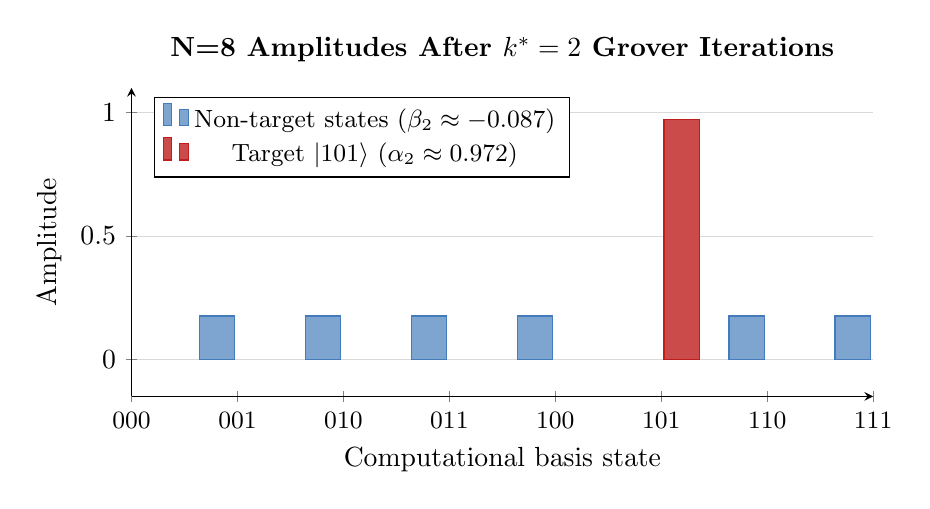
\begin{tikzpicture}
\begin{axis}[
  width=11cm, height=5.5cm,
  ybar, bar width=0.45cm,
  xlabel={Computational basis state},
  ylabel={Amplitude},
  title={\textbf{N=8 Amplitudes After $k^*=2$ Grover Iterations}},
  xtick={0,1,2,3,4,5,6,7},
  xticklabels={000,001,010,011,100,101,110,111},
  xticklabel style={font=\small},
  ymin=-0.15, ymax=1.1,
  ymajorgrids=true, grid style={line width=0.2pt,draw=gray!30},
  axis lines=left, legend pos=north west,
  legend style={font=\small},
]
  \addplot[fill=qblue!55,draw=qblue!80] coordinates
    {(0,0.176)(1,0.176)(2,0.176)(3,0.176)(4,0.176)(6,0.176)(7,0.176)};
  \addplot[fill=qred!80,draw=qred] coordinates {(5,0.972)};
  \legend{Non-target states ($\beta_2\approx-0.087$), Target $\ket{101}$ ($\alpha_2\approx0.972$)}
\end{axis}
\end{tikzpicture}

\vspace{0.4cm}
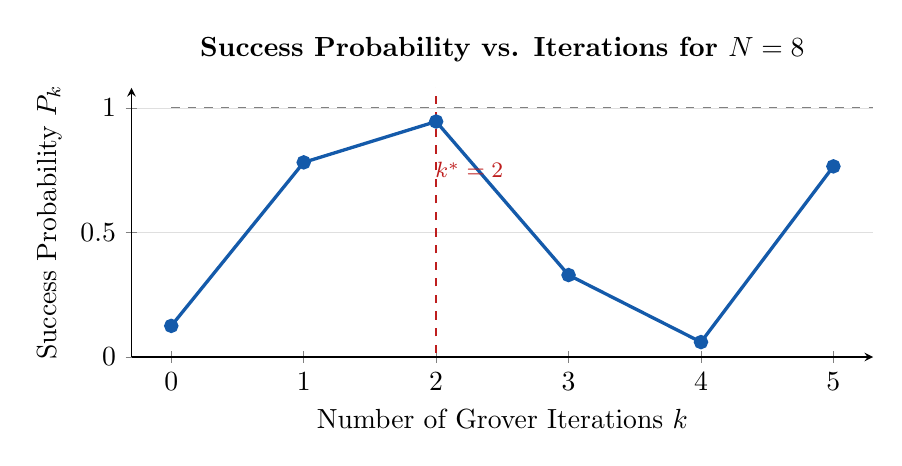
\begin{tikzpicture}
\begin{axis}[
  width=11cm, height=5.0cm,
  xlabel={Number of Grover Iterations $k$},
  ylabel={Success Probability $P_k$},
  title={\textbf{Success Probability vs. Iterations for $N=8$}},
  xmin=-0.3, xmax=5.3, ymin=0, ymax=1.08,
  xtick={0,1,2,3,4,5},
  ymajorgrids=true, grid style={line width=0.2pt,draw=gray!25},
  axis lines=left,
]
  \addplot[qblue,very thick,mark=*,mark options={fill=qblue}] coordinates
    {(0,0.125)(1,0.781)(2,0.945)(3,0.329)(4,0.060)(5,0.765)};
  \addplot[dashed,qred,thick] coordinates {(2,-0.05)(2,1.1)};
  \node[qred,font=\footnotesize] at (axis cs:2.25,0.75) {$k^*=2$};
  \addplot[dashed,gray] coordinates {(0,1)(5.3,1)};
\end{axis}
\end{tikzpicture}
\caption{Top: amplitude bar chart after $k^*=2$ iterations. Bottom: oscillating success probability — stopping at $k^*=2$ gives the first near-maximum.}
\label{fig:ex2}
\end{figure}

%% -----------------------------------------------------------
\subsection{Example 3: $N=16$ ($n=4$ qubits)}

$\theta=\arcsin(1/4)\approx14.48°$, $k^*=\lfloor\frac\pi4\cdot4\rfloor=3$.

\begin{table}[H]
\centering
\begin{tabular}{ccccc}
\toprule
$k$ & $\phi=(2k{+}1)\theta$ & $\alpha_k$ & $\beta_k=\cos\phi/\!\sqrt{15}$ & $P_k$ \\
\midrule
0 & $14.5°$ & $0.250$ & $0.250$ & $6.3\%$ \\
1 & $43.4°$ & $0.687$ & $0.187$ & $47.2\%$ \\
2 & $72.3°$ & $0.953$ & $0.079$ & $90.8\%$ \\
3 & $101.2°$ & $0.981$ & $-0.051$ & $\mathbf{96.2\%}$ \\
4 & $130.1°$ & $0.763$ & $-0.175$ & $58.2\%$ \\
\bottomrule
\end{tabular}
\caption{$N=16$: optimal at $k^*=3$. At $k=4$ the probability drops — clear evidence of over-rotation.}
\end{table}

\begin{figure}[H]
\centering
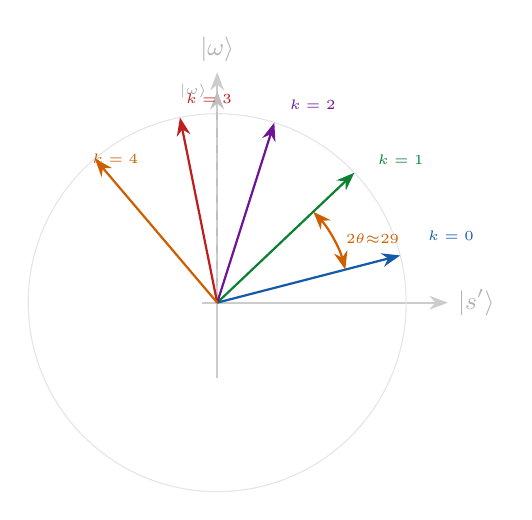
\begin{tikzpicture}[>=Stealth,scale=2.4]
  \draw[->,thick,gray!40] (-0.08,0)--(1.22,0) node[right,gray!60,font=\small]{$\ket{s'}$};
  \draw[->,thick,gray!40] (0,-0.4)--(0,1.22) node[above,gray!60,font=\small]{$\ket\omega$};
  \draw[thin,gray!20] (0,0) circle(1.0);
  \draw[->,thick,black!25,dashed] (0,0)--(0,1.12) node[left,black!35,font=\tiny]{$\ket\omega$};

  \def\th{14.48}
  \foreach \k/\col/\pos in {
      0/qblue/above right,
      1/qgreen/right,
      2/qpurple/right,
      3/qred/right,
      4/qorange/below right}{
    \pgfmathsetmacro{\ang}{(2*\k+1)*\th}
    \draw[->,thick,\col] (0,0)--({cos(\ang)},{sin(\ang)});
    \node[\pos,\col,font=\tiny] at ({1.1*cos(\ang)},{1.1*sin(\ang)}) {$k=\k$};
  }
  % Arc for 2*theta
  \draw[<->,thin,qorange,thick]
    ({0.7*cos(\th)},{0.7*sin(\th)}) arc[start angle=\th,end angle=3*\th,radius=0.7]
    node[midway,right=1pt,qorange,font=\tiny]{$2\theta{\approx}29°$};
\end{tikzpicture}
\caption{$N=16$ geometric view. Each Grover step rotates by $\approx29°$. At $k=3$ the state is closest to $\ket\omega$ ($96.2\%$). At $k=4$ it overshoots.}
\label{fig:ex3_geo}
\end{figure}

%% -----------------------------------------------------------
\subsection{Example 4: $N=64$ ($n=6$ qubits) — Success Probability Curve}

$\theta=\arcsin(1/8)\approx7.18°$, $k^*=\lfloor\frac\pi4\cdot8\rfloor=6$.

\begin{figure}[H]
\centering
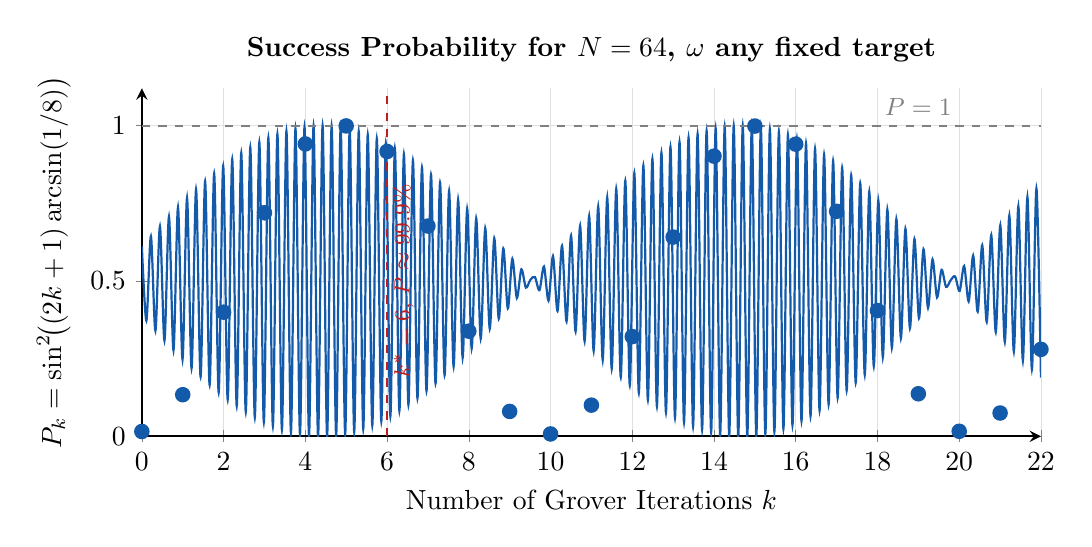
\begin{tikzpicture}
\begin{axis}[
  width=13cm, height=6cm,
  xlabel={Number of Grover Iterations $k$},
  ylabel={$P_k = \sin^2\!\bigl((2k+1)\arcsin(1/8)\bigr)$},
  title={\textbf{Success Probability for $N=64$, $\omega$ any fixed target}},
  domain=0:22, samples=23,
  xmin=0, xmax=22, ymin=0, ymax=1.12,
  xtick={0,2,4,6,8,10,12,14,16,18,20,22},
  ymajorgrids=true, xmajorgrids=true,
  grid style={line width=0.2pt,draw=gray!25},
  axis lines=left, thick,
]
  \addplot[qblue,very thick,mark=*,mark options={fill=qblue,scale=1.1},
           only marks] coordinates {
    (0,0.0156)(1,0.1340)(2,0.3997)(3,0.7197)(4,0.9413)(5,0.9993)(6,0.9170)
    (7,0.6770)(8,0.3386)(9,0.0802)(10,0.0077)(11,0.1005)(12,0.3211)
    (13,0.6415)(14,0.9020)(15,0.9989)(16,0.9406)(17,0.7244)(18,0.4049)
    (19,0.1371)(20,0.0163)(21,0.0751)(22,0.2800)};
  \addplot[qblue,thick,smooth,domain=0:22,samples=200]
    {sin(deg((2*x+1)*asin(0.125)))^2};
  \addplot[dashed,qred,thick] coordinates {(6,0)(6,1.12)};
  \node[qred,font=\footnotesize,rotate=90] at (axis cs:6.4,0.5) {$k^*=6$, $P\approx99.9\%$};
  \addplot[dashed,gray] coordinates {(0,1)(22,1)};
  \node[gray,font=\small] at (axis cs:19,1.06) {$P=1$};
\end{axis}
\end{tikzpicture}
\caption{The success probability oscillates sinusoidally. The first maximum occurs at $k^*=6$ iterations with $P\approx99.9\%$. Note the characteristic periodic over/under-rotation pattern.}
\label{fig:ex4_prob}
\end{figure}

\subsection{Example 5: Multiple Targets ($M > 1$)}

If there are $M$ marked items ($M < N/2$), the analysis extends with:
\[
  \sin\theta_M = \sqrt{\frac{M}{N}}, \qquad
  k^*_M \approx \frac{\pi}{4}\sqrt{\frac{N}{M}}, \qquad
  \text{speedup over classical: }\frac{N/M}{k^*_M} \approx \frac{4}{\pi}\sqrt{\frac{N}{M}}
\]

\begin{exbox}{$N=256$, $M=4$ (4 targets among 256 items)}
\[
  \theta_M = \arcsin\!\sqrt{\tfrac{4}{256}} = \arcsin\!\tfrac{1}{8} \approx 7.18°, \quad
  k^* \approx \tfrac\pi4\sqrt{\tfrac{256}{4}} = \tfrac\pi4\cdot 8 \approx 6 \text{ steps}.
\]
Classical average: $256/(2\cdot4) = 32$ steps. Quantum: $\approx6$ steps. \textbf{Speedup: $\approx5.3\times$}.
\end{exbox}

%% ===========================================================
\section{Full Algorithm Statement}
\label{sec:alg}

\begin{algobox}{Grover's Search Algorithm}
\textbf{Input:} Oracle $U_f$ for $f:\{0,1\}^n\to\{0,1\}$ with unique solution $\omega$; $N=2^n$.\\
\textbf{Output:} $\omega$ with probability $\geq 1-\Order{1/N}$.

\medskip
\begin{enumerate}[leftmargin=2em,label=\textbf{Step \arabic*.}]
  \item \textbf{Initialise.} Prepare $\ket{0}^{\otimes n}\ket{1}$ (data + ancilla).
  \item \textbf{Superpose.} Apply $H^{\otimes n}$ to data and $H$ to ancilla:
        \[
          \ket{s}\ket{-} = \frac{1}{\sqrt{N}}\sum_{x=0}^{N-1}\ket{x}\ket{-}
        \]
  \item \textbf{Iterate $k^*$ times.} For $j = 1, 2, \ldots, k^*$:
        \begin{enumerate}[label=(\alph*)]
          \item Apply $U_f$: phase-flip the target. \hfill \emph{(Oracle query)}
          \item Apply $D = H^{\otimes n}(2\proj{0}-I)H^{\otimes n}$: diffusion.
        \end{enumerate}
        where $k^* = \bigl\lfloor\tfrac{\pi}{4}\sqrt{N}\bigr\rfloor$.
  \item \textbf{Measure} the data register. Output the result.
\end{enumerate}

\medskip
\textbf{Query complexity:} $\Theta(\sqrt{N})$. \quad \textbf{Gate complexity:} $\Order{n\sqrt{N}}$.
\end{algobox}

%% ===========================================================
\section{Complexity and Optimality}
\label{sec:complexity}

\subsection{Query Complexity}

\begin{thmbox}{Query Complexity of Grover's Algorithm}
Grover's algorithm finds the unique marked element with probability $\geq 1-\delta$ using
\[
  Q = \Order{\sqrt{N}\,\log(1/\delta)}
\]
queries to the oracle. For constant success probability, $Q = \Theta(\sqrt{N})$.
\end{thmbox}

\subsection{Classical Lower Bound}

\begin{thmbox}{Classical Lower Bound (trivial)}
Any deterministic or randomised classical algorithm for unstructured search requires $\Omega(N)$ oracle queries in the worst case.\\[4pt]
\textbf{Proof sketch:} After $k < N$ queries on an $N$-element space, at most $k$ items have been checked. The adversary can always place the target among the unchecked items. $\square$
\end{thmbox}

\subsection{Quantum Lower Bound (Grover is Optimal!)}

\begin{thmbox}{Quantum Lower Bound (Bennett–Bernstein–Brassard–Vazirani, 1997)}
Any quantum algorithm for unstructured search requires $\Omega(\sqrt{N})$ oracle queries.\\[4pt]
\textbf{Proof idea (polynomial method):} After $k$ quantum queries, the amplitude of the target state is a degree-$2k$ polynomial in the oracle parameters. For this polynomial to have $\Omega(1)$ magnitude, we need $k = \Omega(\sqrt{N})$ by polynomial approximation theory. $\square$
\end{thmbox}

Thus Grover's algorithm is \textbf{exactly optimal} in the query complexity model.

\subsection{Summary Table}

\begin{table}[H]
\centering
\begin{tabular}{lccc}
\toprule
\textbf{Model} & \textbf{Queries (unique solution)} & \textbf{Queries ($M$ solutions)} & \textbf{Optimal?} \\
\midrule
Classical (worst) & $N$ & $N/M$ & Yes \\
Classical (average) & $N/2$ & $N/(2M)$ & Yes \\
Quantum (Grover) & $\dfrac{\pi}{4}\sqrt{N}$ & $\dfrac{\pi}{4}\sqrt{N/M}$ & \textbf{Yes (proven)} \\
\bottomrule
\end{tabular}
\caption{Query complexity comparison. Grover achieves a tight $\Theta(\sqrt{N/M})$ speedup.}
\end{table}

%% ===========================================================
\section{Common Pitfalls and Practical Notes}
\label{sec:pitfalls}

\begin{keybox}{Pitfall 1 — Over-Rotation}
Applying \emph{more} than $k^*$ iterations \textbf{decreases} the success probability. The state over-rotates past $\ket\omega$. Always compute $k^* = \lfloor\frac\pi4\sqrt{N/M}\rfloor$ carefully.
\end{keybox}

\begin{keybox}{Pitfall 2 — Unknown $M$}
If the number of solutions $M$ is not known, use \textbf{Quantum Counting} (phase estimation on $G$) to estimate $M$, then apply Grover. Alternatively, a randomised strategy: pick $k$ uniformly in $[1,\sqrt{N}]$ and repeat $O(\log(1/\delta))$ times, achieving $O(\sqrt{N})$ expected queries.
\end{keybox}

\begin{keybox}{Pitfall 3 — Not a Speedup for All Problems}
Grover accelerates search and any problem reducible to search by a quadratic factor. It does \emph{not} provide exponential speedup. Problems with classical $O(\text{poly}(n))$ algorithms do not become fundamentally easier.
\end{keybox}

\begin{notebox}
\textbf{Verification.} After the quantum circuit outputs a candidate $x$, verify classically in $O(1)$ by evaluating $f(x)$. If wrong (probability $\approx 1/N$), repeat the entire procedure.
\end{notebox}

\subsection{Gate Count for the Diffusion Operator}

The multi-controlled phase flip $(2\proj{0}-I)$ on $n$ qubits can be decomposed as:
\[
  2\proj{0}-I = X^{\otimes n}\cdot C^{n-1}Z \cdot X^{\otimes n}
\]
where $C^{n-1}Z$ is an $(n-1)$-controlled $Z$ gate. This requires $O(n)$ gates using ancilla-based decompositions. Thus each diffusion step uses $O(n)$ elementary gates, and the total gate count of Grover's algorithm is:
\[
  \text{Total gates} = k^*\times\bigl(O(n) + \text{cost}(U_f)\bigr) \approx \frac\pi4\sqrt{N}\cdot O(n)
\]

%% ===========================================================
\section{Generalisation: Amplitude Amplification}
\label{sec:ampamp}

Grover's algorithm is a special case of the much more general \textbf{Amplitude Amplification} framework due to Brassard, Høyer, Mosca, and Tapp (2002).

\begin{defbox}{Amplitude Amplification}
Let $A$ be any quantum algorithm on $n+m$ qubits. Say a basis state $\ket{x,y}$ is \textbf{good} if $f(x)=1$. Let $a = \|P_{\rm good}A\ket{0}\|^2$ be the probability that $A$ produces a good state. Define:
\[
  Q = -A S_0 A^\dagger S_{\rm good}
\]
where $S_0 = I - 2\proj{0^{n+m}}$ and $S_{\rm good}$ flips the phase of good states. Then $k$ applications of $Q$ give success probability $\sin^2((2k+1)\arcsin\sqrt{a})$.
\end{defbox}

Grover's algorithm is the special case $A = H^{\otimes n}$, giving $a=M/N$.

\textbf{Consequence:} If any classical algorithm solves a problem with probability $p$, its quantum analogue (using amplitude amplification) solves it in $O(1/\sqrt{p})$ quantum steps instead of $O(1/p)$ classical steps — always a quadratic speedup.

%% ===========================================================
\section{Summary}
\label{sec:summary}

\begin{algobox}{Lecture Summary}
\begin{enumerate}[leftmargin=1.5em]
  \item \textbf{Problem:} Unstructured search over $N=2^n$ items. Classical: $\Theta(N)$; Quantum: $\Theta(\sqrt N)$.

  \item \textbf{Oracle:} Phase oracle $U_f = I-2\proj\omega$ phase-flips only the target $\ket\omega$. Built via \emph{phase kick-back} from the standard oracle.

  \item \textbf{Diffusion:} $D = 2\proj s - I$ inverts amplitudes about their mean. Implemented as $H^{\otimes n}(2\proj 0 - I)H^{\otimes n}$.

  \item \textbf{Geometric view:} $G = D\cdot U_f$ rotates the state by $2\theta$ per step inside the 2D plane $\mathrm{span}\{\ket\omega,\ket{s'}\}$.

  \item \textbf{Algebraic view:} Amplitudes satisfy $\alpha_k = \sin((2k+1)\theta)$, $\beta_k = \cos((2k+1)\theta)/\!\sqrt{N-1}$. Both views are equivalent.

  \item \textbf{Optimal iterations:} $k^* \approx \frac\pi4\sqrt{N/M}$ gives $P(\text{success})\approx 1$.

  \item \textbf{Optimality:} Proven $\Omega(\sqrt N)$ lower bound; Grover is tight.
\end{enumerate}
\end{algobox}

\subsection*{Review Questions}

\begin{enumerate}
  \item Derive the phase kick-back trick from first principles. Why must the ancilla be in $\ket{-}$?
  \item Show algebraically that $D = 2\proj s - I$ performs inversion about the mean on the amplitudes.
  \item For $N=256$ with one target, compute $k^*$ and the exact success probability $P_{k^*}$.
  \item Explain geometrically \emph{why} over-rotation reduces the success probability.
  \item Prove that the matrix $M$ in the amplitude recurrence has eigenvalues $e^{\pm 2i\theta}$.
  \item For $N=1024$, $M=16$ targets: how many Grover iterations are needed? What is the speedup over classical?
  \item Describe the amplitude amplification framework and state how it generalises Grover's algorithm.
  \item Why does Grover's algorithm give only a \emph{quadratic} speedup, not an exponential one? What is fundamentally different from Shor's algorithm?
\end{enumerate}

\subsection*{Further Reading}

\begin{itemize}
  \item L.\,K.\,Grover, ``A fast quantum mechanical algorithm for database search,'' \textit{Proceedings of ACM STOC}, 1996.
  \item C.\,H.\,Bennett, E.\,Bernstein, G.\,Brassard, U.\,Vazirani, ``Strengths and weaknesses of quantum computing,'' \textit{SIAM Journal on Computing} 26(5), 1997.
  \item G.\,Brassard, P.\,Høyer, M.\,Mosca, A.\,Tapp, ``Quantum amplitude amplification and estimation,'' \textit{AMS Contemporary Mathematics} 305, 2002.
  \item M.\,A.\,Nielsen \& I.\,L.\,Chuang, \textit{Quantum Computation and Quantum Information}, Cambridge University Press, Chapter 6.
  \item R.\,de Wolf, \textit{Quantum Computing: Lecture Notes} (freely available at \texttt{arxiv.org/abs/1907.09415}).
\end{itemize}

\end{document}
